\documentclass[12pt]{article}
\usepackage{textcomp}
\usepackage{ucs}
\usepackage[utf8x]{inputenc}
\usepackage[T1]{fontenc}   
\usepackage[french]{babel} 
\usepackage{array}
\usepackage{amsmath}
\usepackage{supertabular}
\usepackage{graphicx}
\usepackage{hyperref}
\usepackage{float}
%\usepackage{fullpage}

\title{LELEC1930 \hspace{0.5cm} Introduction aux télécommunications\\ \large Notes supplémentaires}
\author{Fastré Ludovic}
\date{\today}


\begin{document}
\maketitle

\tableofcontents 

\newpage

\section{Lignes}

\subsection{Atténuation}

L’atténuation ou affaiblissement est la diminution de l'amplitude ou de la puissance d'une onde ou d'un signal au cours de sa transmission. On la quantifie par le rapport entre leur grandeur à la sortie par celui à l'entrée de la section considérée. Ce rapport, toujours inférieur à 1 par définition, s'exprime souvent en décibels quand il s'agit de puissance ou de valeur efficace.

\begin{center}
Atténuation = $\frac{\text{valeur en sortie}}{\text{valeur en entrée}}$\\
\vspace{2 mm}
Atténuation = $10log(\frac{\text{valeur en sortie}}{\text{valeur en entrée}}) (dB)$
\end{center}

\subsection{Distorsion}

On appelle distorsion dans un appareil ou un canal de transmission l'ensemble des modifications indésirables d'un signal qui ne soient ni un gain, ni une atténuation, ni un retard.

\subsection{Effet pelliculaire}

A fréquence élevée, le courant a tendance à ne circuler qu'en surface des conducteurs (matériau permettant des échanges d'énergie entre deux systèmes). Il provoque la décroissance de la densité de courant à mesure que l'on s'éloigne de la périphérie du conducteur. Il en résulte une augmentation de la résistance du conducteur.

\begin{figure}[H]
\centering
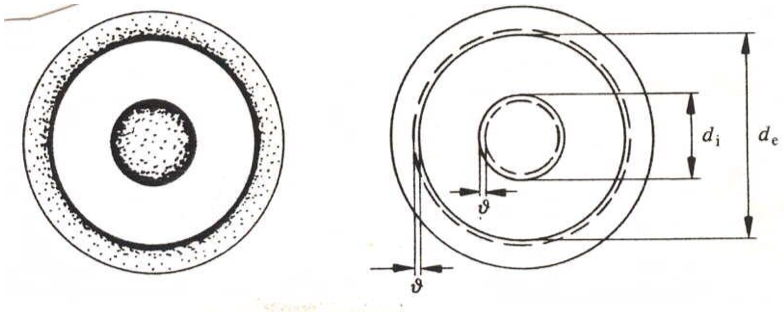
\includegraphics[scale=0.5]{images/EffetPelliculaire.png}
\end{figure}

\subsection{Dispersion}

C'est le phénomène affectant une onde se propageant dans un milieu dit « dispersif », c'est-à-dire dans lequel les différentes fréquences constituant l'onde ne se propagent pas à la même vitesse. Tous les milieux sont dispersifs en plus ou moins grande proportion. Seul le vide n'est pas dispersif.

\subsection{Impédance}

L'impédance mesure l'opposition d'un circuit électrique au passage d'un courant alternatif sinusoïdal.

\subsubsection{Loi d'ohm généralisée}

La tension aux bornes d'une impédance est égale au produit de l'impédance par le courant :
\begin{center}
$ V_z=Z\,I_z\,  $\\
Z = « Résistance complexe équivalente »
\end{center}

\subsection{Pupinisation}

Technique visant à supprimer les parasites haute fréquence et à assurer un affaiblissement du signal indépendant de la fréquence en introduisant des bobines d'inductance dans les lignes téléphoniques.

\subsection{Diaphonie}

On nomme diaphonie (parfois « bruit » ou « crosstalk » en anglais) l'interférence d'un premier signal avec un second. On trouve des traces du premier signal, dans le signal du second, souvent à cause de phénomènes d'induction électromagnétique.

\newpage

\section{Propagation et antennes}

\subsection{Onde directe}

Onde qui se propage linéairement.
\begin{itemize}
\item En ligne droite
\item Portée limitée (horizon)
\item Interférence avec onde réfléchie
\end{itemize}

\begin{figure}[H]
\centering
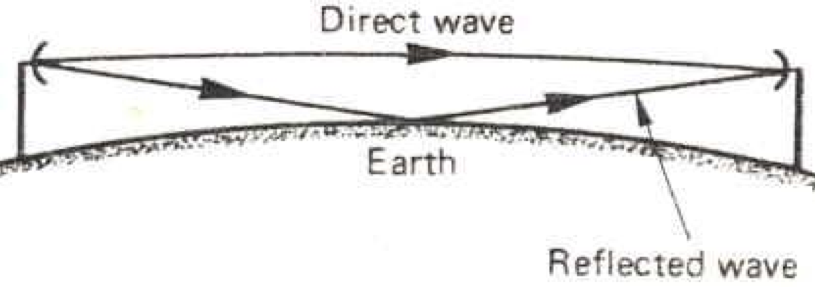
\includegraphics[scale=0.5]{images/OndeDirecte.png}
\end{figure}

\subsection{Onde de sol}

Les ondes de sol, comme leur nom l’indique, voyagent à la surface de la Terre C'est une onde de basse fréquence généralement utilisée pour les radio am.

\begin{figure}[H]
\centering
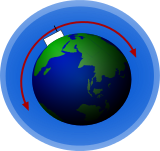
\includegraphics[scale=0.8]{images/OndeDeSol.png}
\end{figure}

\subsection{Propagation ionosphérique}

On appelle propagation ionosphérique la propriété des ondes électromagnétiques de parcourir des distances plus grandes que la simple ligne de vue par réflexion sur l’ionosphère.

\begin{figure}[H]
\centering
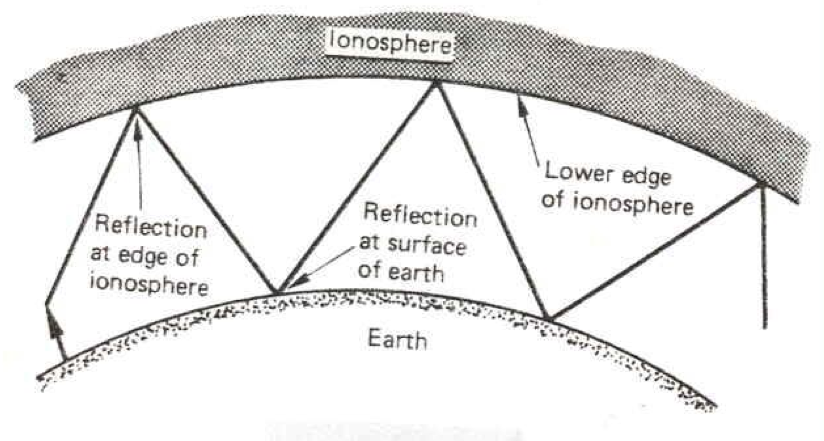
\includegraphics[scale=0.4]{images/PropagationIono.png}
\end{figure}

\subsection{Satellite géostationnaire}

Satellite se trouvant à 35 784 km d'altitude au-dessus de l'équateur de la Terre. Sur cette orbite le satellite se déplace de manière exactement synchrone avec la planète et reste constamment au-dessus du même point de la surface.

\begin{figure}[H]
\centering
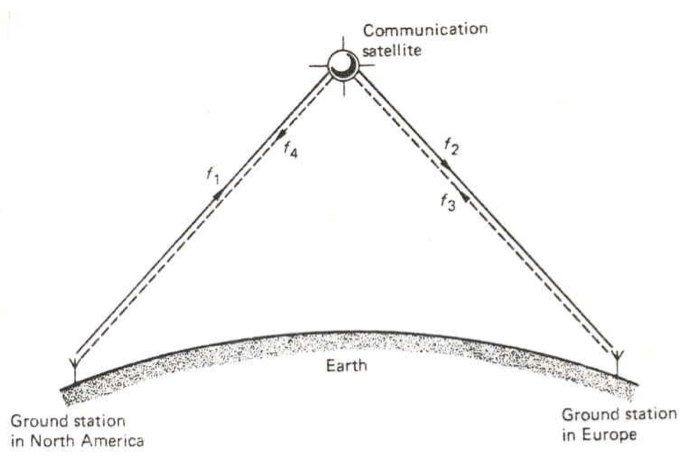
\includegraphics[scale=0.4]{images/SatelliteGeo.png}
\end{figure}

\subsection{Effet Doppler}

L'effet Doppler (distorsion) est le décalage de fréquence d’une onde entre la mesure à l'émission et la mesure à la réception lorsque la distance entre l'émetteur et le récepteur varie au cours du temps.

\subsection{Gain}

\begin{center}
$ \frac{\text{Puissance dans direction de puissance maximum}}{\text{Puissance dans cette direction si l'antenne était isotrope}} $
\end{center}

\subsection{Angle d'ouverture}

L'angle d'ouverture d'une antenne est l'angle de direction pour lequel la puissance rayonnée est la moitié de la puissance rayonnée dans la direction la plus favorable. 

\subsection{Antenne dipolaire}

L'antenne dipolaire est une antenne demi-onde au centre de laquelle est raccordée la ligne d'alimentation.

\subsection{Antenne endfire}

L'antenne endfire est une antenne consistant en un fil conducteur enroulé sous la forme d'une hélice.

\subsection{Antenne Yagi}

L'antenne Yagi est une antenne à éléments parasites utilisable des HF aux UHF. Elle peut être assimilée à une antenne réseau dont les éléments seraient alimentés par induction mutuelle. Si les espacements et longueurs des brins sont optimaux, le diagramme de rayonnement et le gain est celui d'un réseau.

\begin{figure}[H]
\centering
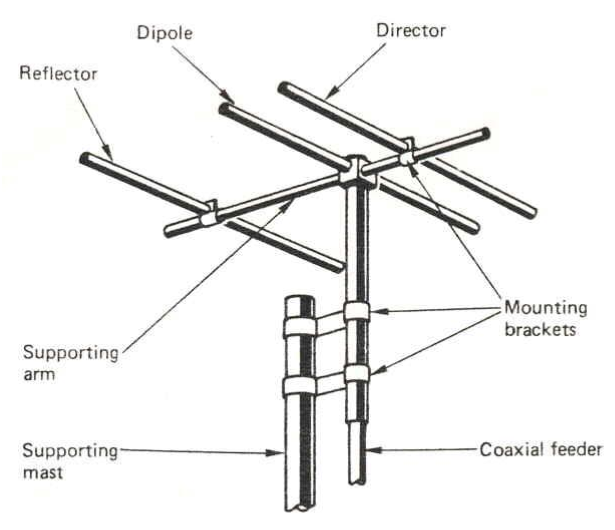
\includegraphics[scale=0.3]{images/Yagi.png}
\end{figure}

\subsection{Antenne parabolique}

L'antenne parabolique est une antenne disposant d'un réflecteur paraboloïdal, basé sur les propriétés géométriques de la courbe nommée parabole. Cette antenne qualifiée d'universelle puisqu'elle fonctionne en théorie sur n'importe quelle fréquence ou longueur d'onde. Le réflecteur parabolique est chargé de concentrer les ondes reçues ou émises (radar, télévision, ISM et Wi-Fi, radio-amateurisme, faisceaux hertziens, ou ondes émises par les astres en radioastronomie) vers l'antenne-source, qui se situe au foyer de la parabole.

\section{Modulations}

\end{document}